\note{Now lets talk about the physics of some common featureless phases}
\begin{frame}{Magnetization/Density Plateaus}
\vskip-1.5cm
Stable featureless insulators form magnetization or density plateaus

Example Hamiltonians and phase diagrams:
\only<1>{
\begin{block}{Band Insulators}
\vskip-0.5cm
$$
H_{FF} =  \sum\limits_{<ij>}-t_{ij} c^{\dagger}_i c_j - \mu \sum\limits_i N_i 
$$
\end{block}
\begin{columns}[T]
    \begin{column}[T]{.45\textwidth}
        \vskip-1cm
        \begin{figure}
        \centering
        \scalebox{0.7}{
         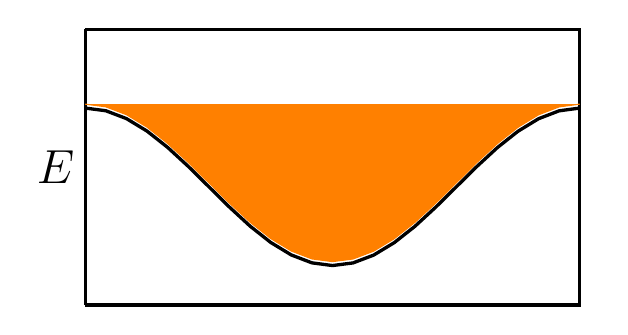
\begin{tikzpicture}[domain=0:6.28]
      \draw[very thick] (0, -2.5) -- (0,1) node[left, midway] {\LARGE $E$} ;
      \draw[very thick] (0, 1)-- (6.28,1) -- (6.28, -2.5) -- (0, -2.5);
      \draw[color=black, very thick] plot (\x,{-1+cos(\x r)}) node[right] {};
      \draw[color=orange, fill] plot (\x,{-0.95+cos(\x r)}) {};
  \end{tikzpicture}
  
        }
        \end{figure}
    \end{column}
    \begin{column}[T]{.55\textwidth}
    \vskip-0.7cm
    \bi 
    \item Symmetry protected band touchings can constrain existence of a band insulator
    \note{beyond integer filling LSM, on a given lattice tight-bonding model}
    \item Topological invariants can distinguish different types of band insulators
    \item Some invariants only make sense in the presence of additional symmetries ($\mathcal{T}, \mathcal{C}, \mathcal{I}$)
    \ei
    \end{column}
\end{columns}
}
\only<2>{
\begin{block}{Bose-Hubbard model}
\vskip-0.5cm
$$
H_{BH} = -J \sum\limits_{<ij>} b^{\dagger}_i b_j - \mu \sum\limits_i N_i + \frac12 V \sum\limits_i N_i (N_i-1)
$$
\end{block}
\begin{columns}[T]
    \begin{column}[T]{.45\textwidth}
        \vskip-1.2cm
        \begin{figure}
        \centering
        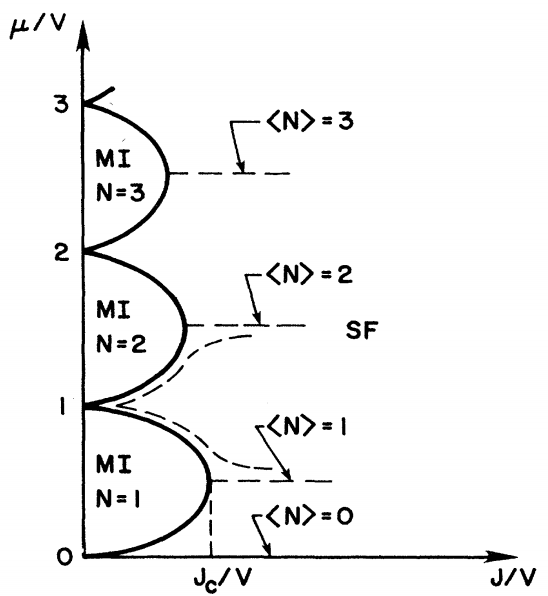
\includegraphics[width=4.5cm]{diagrams/bosehubbard2.png}
        \end{figure}
    \end{column}
    \begin{column}[T]{.55\textwidth}
    \vskip-0.7cm
    \bi 
    \item Interactions are always needed to stop Bose condensation
    \item Unlike free-fermions, not obvious how to construct fractional site filling insulators
    \item Tensor network states give us access to needed construction and to interacting invariants.
    \note{LSM inspired invariants}
    \ei
    \end{column}
\end{columns}
}

\only<3>{
\begin{block}{Haldane Phase for Spin-1 chains $(j=1, m=0)$}
\vskip-0.8cm
$$
H_{AKLT} = \sum\limits_{i} J \vec{S}_i\cdot \vec{S}_{i+1} + J' (\vec{S}_i\cdot \vec{S}_{i+1})^2 + D (S^z_i)^2+BS^x
$$
\end{block}
\begin{columns}[T]
    \begin{column}[T]{.45\textwidth}
        \vskip-1.2cm
        \begin{figure}
        \centering
        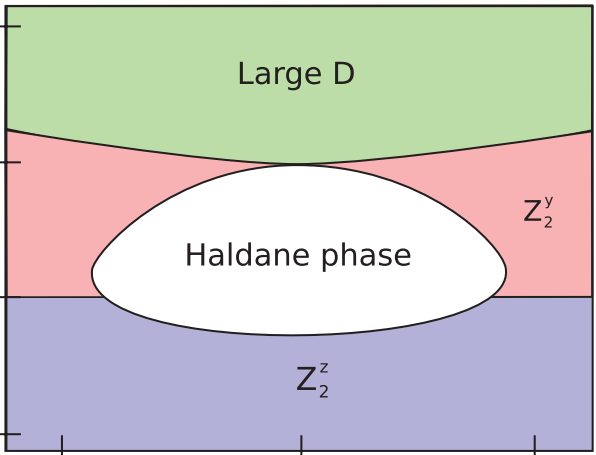
\includegraphics[width=\columnwidth]{diagrams/aklt2.png}
        \end{figure}
    \end{column}
    \begin{column}[T]{.55\textwidth}
    \vskip-0.8cm
    Two distinct featureless insulators:
    \bi 
    \item Large-D phase
    \bi 
    \item Contains product state wavefunction $\ket{\psi} = \ket{000...}$ 
    \ei
    \item Haldane phase
    \bi 
    \item Contains AKLT wavefunction $\ket{\psi} = \Sigma\ket{+00-0+...}$
    \ei 
        \begin{figure}[h]
            \hspace{-2cm}
            \scalebox{1.2}{
            \begin{frame}{MPS Example: AKLT State}
\vskip-1.5cm
\begin{block}{Haldane Phase for Spin-1 chains $(j=1, m=0)$}
\vskip-0.8cm
$$
H_{AKLT} = \sum\limits_{i} J \vec{S}_i\cdot \vec{S}_{i+1} + J' (\vec{S}_i\cdot \vec{S}_{i+1})^2 + D (S^z_i)^2+BS^x
$$
\end{block}
\begin{columns}[T]
    \begin{column}[T]{.45\textwidth}
        \vskip-1.2cm
        \begin{figure}
        \centering
        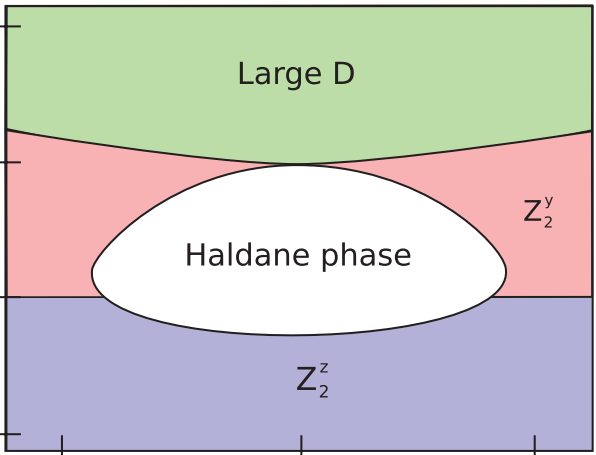
\includegraphics[width=\columnwidth]{diagrams/aklt2.png}
        \end{figure}
    \end{column}
    \begin{column}[T]{.55\textwidth}
    \vskip-0.8cm
    Two distinct featureless insulators:
    \bi 
    \item Large-D phase
    \bi 
    \item Contains product state wavefunction $\ket{\psi} = \ket{000...}$ 
    \ei
    \item Haldane phase
    \bi 
    \item Contains AKLT wavefunction $\ket{\psi} = \Sigma\ket{+00-0+...}$
    \ei 
        \begin{figure}[h]
            \hspace{-2cm}
            \scalebox{1.2}{
            \begin{frame}{MPS Example: AKLT State}
\vskip-1.5cm
\begin{block}{Haldane Phase for Spin-1 chains $(j=1, m=0)$}
\vskip-0.8cm
$$
H_{AKLT} = \sum\limits_{i} J \vec{S}_i\cdot \vec{S}_{i+1} + J' (\vec{S}_i\cdot \vec{S}_{i+1})^2 + D (S^z_i)^2+BS^x
$$
\end{block}
\begin{columns}[T]
    \begin{column}[T]{.45\textwidth}
        \vskip-1.2cm
        \begin{figure}
        \centering
        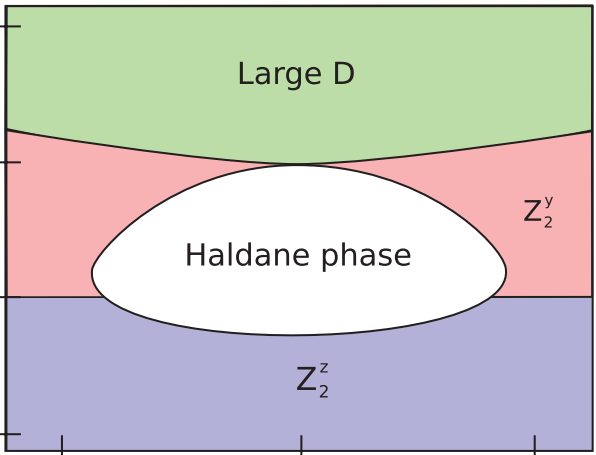
\includegraphics[width=\columnwidth]{diagrams/aklt2.png}
        \end{figure}
    \end{column}
    \begin{column}[T]{.55\textwidth}
    \vskip-0.8cm
    Two distinct featureless insulators:
    \bi 
    \item Large-D phase
    \bi 
    \item Contains product state wavefunction $\ket{\psi} = \ket{000...}$ 
    \ei
    \item Haldane phase
    \bi 
    \item Contains AKLT wavefunction $\ket{\psi} = \Sigma\ket{+00-0+...}$
    \ei 
        \begin{figure}[h]
            \hspace{-2cm}
            \scalebox{1.2}{
            \begin{frame}{MPS Example: AKLT State}
\vskip-1.5cm
\begin{block}{Haldane Phase for Spin-1 chains $(j=1, m=0)$}
\vskip-0.8cm
$$
H_{AKLT} = \sum\limits_{i} J \vec{S}_i\cdot \vec{S}_{i+1} + J' (\vec{S}_i\cdot \vec{S}_{i+1})^2 + D (S^z_i)^2+BS^x
$$
\end{block}
\begin{columns}[T]
    \begin{column}[T]{.45\textwidth}
        \vskip-1.2cm
        \begin{figure}
        \centering
        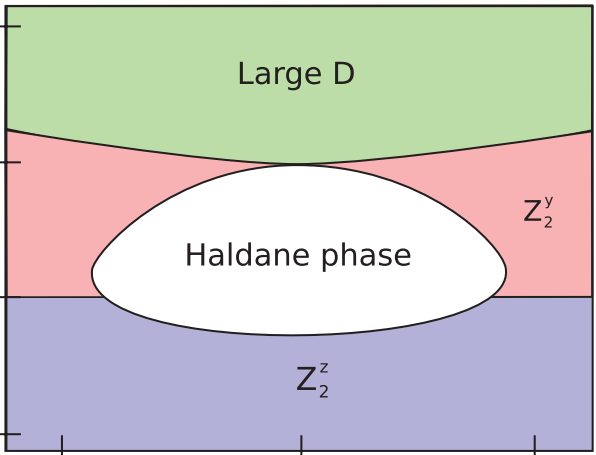
\includegraphics[width=\columnwidth]{diagrams/aklt2.png}
        \end{figure}
    \end{column}
    \begin{column}[T]{.55\textwidth}
    \vskip-0.8cm
    Two distinct featureless insulators:
    \bi 
    \item Large-D phase
    \bi 
    \item Contains product state wavefunction $\ket{\psi} = \ket{000...}$ 
    \ei
    \item Haldane phase
    \bi 
    \item Contains AKLT wavefunction $\ket{\psi} = \Sigma\ket{+00-0+...}$
    \ei 
        \begin{figure}[h]
            \hspace{-2cm}
            \scalebox{1.2}{
            \input{diagrams/aklt.tex}
            }
        \end{figure}

    \ei
    \end{column}
\end{columns}

\end{frame}
            }
        \end{figure}

    \ei
    \end{column}
\end{columns}

\end{frame}
            }
        \end{figure}

    \ei
    \end{column}
\end{columns}

\end{frame}
            }
        \end{figure}

    \ei
    \end{column}
\end{columns}
}
% \only<3>{
% \bi
% \item Spin 3/2 Haldane Phase
% \ei
% $$
% H_{AKLT} = 
% $$
% \begin{figure}
% \centering
% \end{figure}
% }
\end{frame}